
\documentclass[xcolor = dvipsnames]{beamer}
\usetheme{Madrid}
\useoutertheme{infolines} % Alternatively: miniframes, infolines, split
\useinnertheme{circles}
\definecolor{UBCblue}{rgb}{0.04706, 0.13725, 0.26667}
\usecolortheme[named=UBCblue]{structure}

\usepackage{setspace}
\usepackage{gensymb}
\usepackage{caption}
%\usepackage{multirow}
%\usepackage{multicolumn}
%\usepackage{subcaption}
%\doublespacing
\singlespacing
\usepackage{csvsimple}
\usepackage{amsmath}
\usepackage{multicol}
%\usepackage{enumerate}
\usepackage{amssymb}
%\usepackage{graphicx}
\usepackage{newfloat}
%\usepackage{syntax}
\usepackage{listings}
\usepackage{enumitem}
%\usepackage{iithtlc}
\usepackage{color}
\usepackage{tikz}
\usetikzlibrary{shapes,arrows}



%\usepackage{graphicx}
%\usepackage{amssymb}
%\usepackage{relsize}
%\usepackage[cmex10]{amsmath}
%\usepackage{mathtools}
%\usepackage{amsthm}
%\interdisplaylinepenalty=2500
%\savesymbol{iint}
%\usepackage{txfonts}
%\restoresymbol{TXF}{iint}
%\usepackage{wasysym}
\usepackage{amsthm}
\usepackage{mathrsfs}
\usepackage{txfonts}
\usepackage{stfloats}
\usepackage{cite}
\usepackage[bottom]{footmisc}
\usepackage{cases}
\usepackage{mathtools}
\usepackage{caption}
\usepackage{enumerate}	
\usepackage{enumitem}
\usepackage{amsmath}
%\usepackage{xtab}
\usepackage{longtable}
\usepackage{multirow}
%\usepackage{algorithm}
%\usepackage{algpseudocode}
\usepackage{enumitem}
\usepackage{mathtools}
\usepackage{hyperref}
%\usepackage[framemethod=tikz]{mdframed}
\usepackage{listings}
    %\usepackage[latin1]{inputenc}                                 %%
    \usepackage{color}                                            %%
    \usepackage{array}                                            %%
    \usepackage{longtable}                                        %%
    \usepackage{calc}                                             %%
    \usepackage{multirow}                                         %%
    \usepackage{hhline}                                           %%
    \usepackage{ifthen}                                           %%
  %optionally (for landscape tables embedded in another document): %%
    \usepackage{lscape}     


\usepackage{url}
\def\UrlBreaks{\do\/\do-}


%\usepackage{stmaryrd}


%\usepackage{wasysym}
%\newcounter{MYtempeqncnt}
\DeclareMathOperator*{\Res}{Res}
%\renewcommand{\baselinestretch}{2}
\renewcommand\thesection{\arabic{section}}
\renewcommand\thesubsection{\thesection.\arabic{subsection}}
\renewcommand\thesubsubsection{\thesubsection.\arabic{subsubsection}}

%\renewcommand\thesectiondis{\arabic{section}}
%\renewcommand\thesubsectiondis{\thesectiondis.\arabic{subsection}}
%\renewcommand\thesubsubsectiondis{\thesubsectiondis.\arabic{subsubsection}}

% correct bad hyphenation here
\hyphenation{op-tical net-works semi-conduc-tor}

%\lstset{
%language=C,
%frame=single, 
%breaklines=true
%}

%\lstset{
	%%basicstyle=\small\ttfamily\bfseries,
	%%numberstyle=\small\ttfamily,
	%language=Octave,
	%backgroundcolor=\color{white},
	%%frame=single,
	%%keywordstyle=\bfseries,
	%%breaklines=true,
	%%showstringspaces=false,
	%%xleftmargin=-10mm,
	%%aboveskip=-1mm,
	%%belowskip=0mm
%}

%\surroundwithmdframed[width=\columnwidth]{lstlisting}
\def\inputGnumericTable{}                                 %%
\lstset{
%language=C,
frame=single, 
breaklines=true,
columns=fullflexible
}


\begin{document}
\title{\textbf{EE2230 Power electronics}}   
\author{\textit{Raktim Gautam Goswami (EE17BTECH11051) \newline Adarsh Bandi (CE17BTECH11010)}
\linebreak 
\linebreak Group 36}

\frame{\titlepage} 

\frame{\frametitle{Table of contents}\tableofcontents} 


\section{Problem statement } 
\frame{\frametitle{Problem statement}
\textbf{Problem 4.1} Observe the output of the Source pin of the n-MOS on oscilloscope and write python script to generate the same.
}


\section{Solution}
\frame{\frametitle{Solution}
\textbf{Explanation:} 
\text   Below is the pinout diagram of n-MOS(IRF 540) 

\begin{figure}[!h]
\begin{center}
\includegraphics[width=0.4\columnwidth]{./Figs/fig1.png}
\end{center}
\end{figure}
}

\begin{frame}
\textbf{Explanation contd.}
\linebreak
\linebreak
\begin{flushleft}
We connect the source pin of n-MOS with the pin5 of TLP350(accoridng to the connections mentioned in manual).
\linebreak
\linebreak
\textbf{}TLP350 is a power amplifier that accepts low power input and produces high current input to the n-MOS(IRF 540)
\linebreak
\linebreak
\textbf{}The ouput shown on the oscilloscope is of a square  wave pulse with amplitude of 10 and time period of 0.2 msec.

\end{flushleft}
\end{frame}



\section{Figure}
\frame{\frametitle{Figure}

\begin{figure}[!h]
\begin{center}
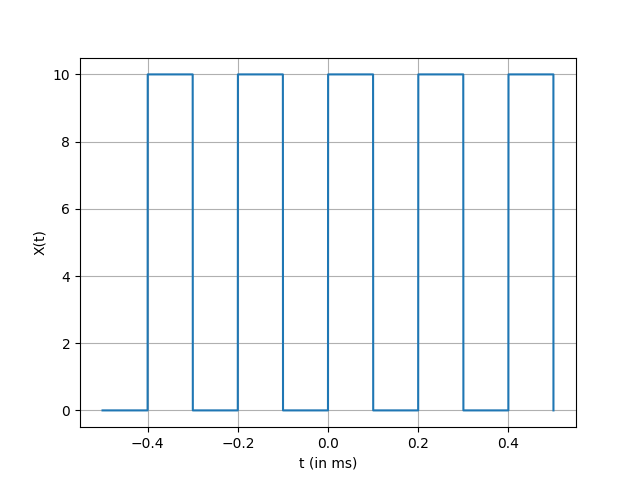
\includegraphics[width=0.7\columnwidth]{./Figs/p1.png}
\end{center}
\caption{Output of the source pin}
\label{fig:}
\end{figure}

}

\section{Code}
\frame{\frametitle{Code}

\href{https://github.com/raktimgg/Power-Electronics/blob/master/Presentation1/p1.py}{https://github.com/raktimgg/Power-Electronics/blob/master/Presentation1/p1.py}

}


\end{document}
